\chapter{Introducción a los sistemas operativos}
\section{
Introducción
}
Es necesario comprender que la actividad informática se centra en un elemento físico\cite{introsistema}, esto es, un equipo de cómputo.

Entre los equipos de cómputo, podemos citar:
\begin{itemize}
	\item  Computadora o PC
	\item Tablets
	\item Teléfonos inteligentes (\textit{smartphones})
\end{itemize}


Estos equipos de cómputo (en adelante, computadoras) son máquinas de origen electrónico con una o más unidades de proceso, además de otros componentes periféricos controlados por programas almacenados en su memoria. Pueden realizar una gran variedad de trabajos.

A todo componente físico de una computadora, es decir, todo aquel componente con el cual podemos interactuar físicamente, se le denomina \textit{\textbf{hardware}}.

Todo \textbf{\textit{hardware}} de una computadora necesita de información que le indique cómo funcionar. Su funcionamiento está definido por instrucciones (programas), que constituyen su soporte lógico (\textbf{\textit{software}}). 

El \textit{software} incluye tanto el sistema operativo como las aplicaciones que utilizamos para realizar tareas específicas. Sin \textit{software}, el \textit{hardware} no podría realizar ninguna operación útil.



\section{Sistema Operativo. Concepto}
Al comprender que el sistema operativo constituye un software, podemos definirlo de la siguiente forma:
\begin{tcolorbox}
	Un \textbf{Sistema Operativo }es el soporte lógico que controla el funcionamiento del equipo físico\cite{introsistema}.
\end{tcolorbox}
Dependiendo el punto de vista, podemos encontrar otras definiciones de un sistema operativo:

\begin{itemize}
	\item  \subsection{Punto de vista del USUARIO}
		\begin{tcolorbox}
			Un \textbf{Sistema Operativo }es un conjunto de programas y funciones que ocultan los detalles del hardware\cite{introsistema}, facilitando al usuario el acceso al mismo. 
	\end{tcolorbox}
	La ocultación de los detalles del hardware persigue dos objetivos:
	    \begin{itemize}
			\item \textbf{Abstracción:} El sistema operativo proporciona una interfaz simplificada que permite a los usuarios y a los desarrolladores de software interactuar con el hardware sin necesidad de conocer su funcionamiento interno. Esto se logra a través de la creación de capas de abstracción que ocultan la complejidad del hardware y presentan una interfaz más amigable y coherente.
			\item \textbf{Seguridad:} El sistema operativo implementa mecanismos de protección para asegurar que los recursos del sistema sean utilizados de manera controlada y segura. Esto incluye la gestión de permisos de acceso, la protección de la memoria, y la prevención de interferencias entre procesos, garantizando así la estabilidad y la integridad del sistema.
		\end{itemize}
	\item \subsection{Punto de vista de GESTOR DE RECURSOS}
	
		\begin{tcolorbox}
			Un \textbf{Sistema Operativo }es el administrador de recursos ofrecidos por el hardware para alcanzar un eficaz rendimiento de los mismos\cite{introsistema}.
		\end{tcolorbox}

	Los recursos fundamentales que administra son:
	
		\begin{itemize}
			\item El procesador.
			\item La memoria
			\item La entrada/salida.
			\item La información.
		\end{itemize}

	
\end{itemize}

	Basado en las definiciones mencionadas, podemos concluir que:
	
	
	\begin{tcolorbox}
		Un \textbf{Sistema Operativo }es un conjunto de programas relacionados entre si, que contribuyen a que la computadora lleve a cabo correctamente su trabajo\cite{introsistema}.
	\end{tcolorbox}
	
	Además podemos afirmar que los sistemas operativos tienen dos objetivos fundamentales:
\begin{itemize}
	\item Facilitar el trabajo al usuario.
	\item Gestionar de forma eficiente los recursos.
\end{itemize}

\section{Evolución histórica.}
A lo largo de la historia, las computadoras evolucionaron de manera espectacular, las primeras máquinas de cómputo carecían de sistema operativo y equipos de tamaño de una sala. Se describen como los sistemas operativos están estrechamente relacionados con la evolución de las computadoras.



\subsection{La primera generación (1945 a 1955): tubos de vacío}

Las primeras computadoras fueron construidas a partir de tubos de vacío, eran voluminosas y consumían mucha energía.
\begin{figure}[H]
	\centering
	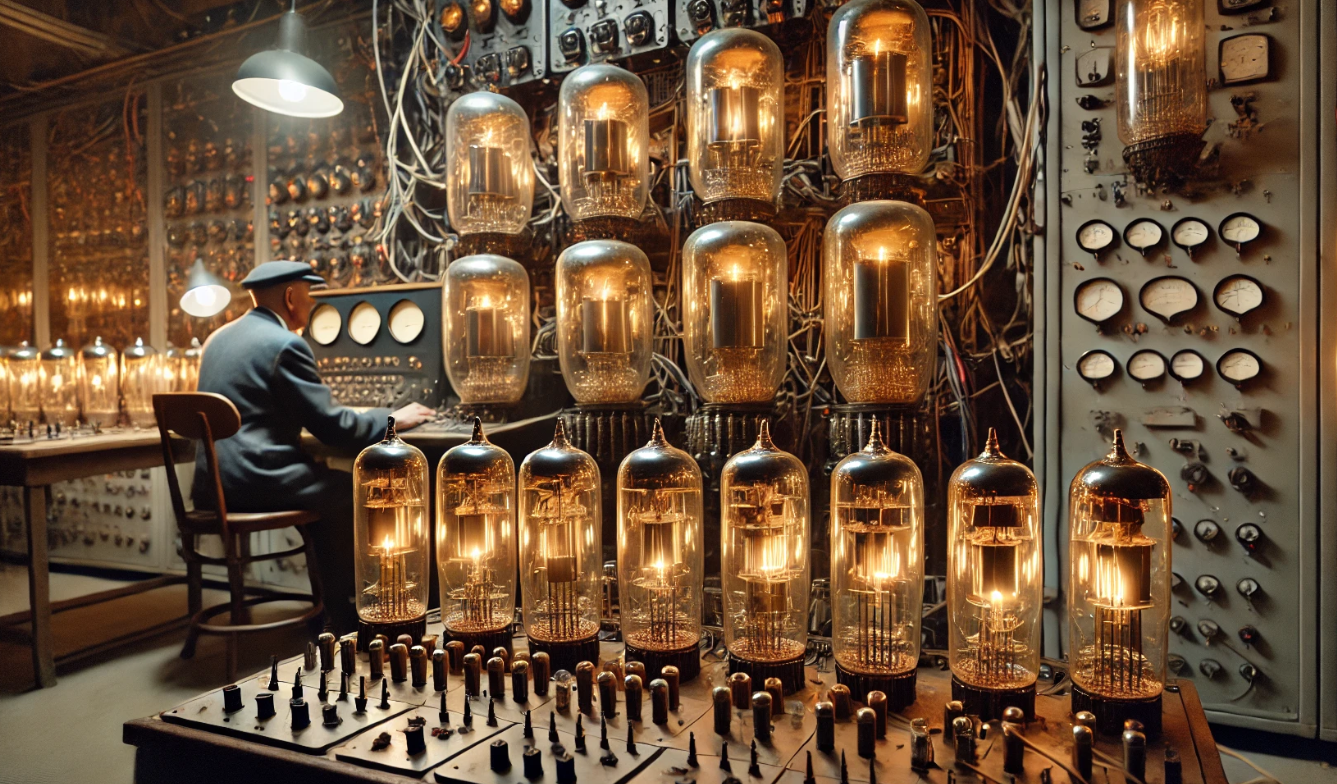
\includegraphics[width=0.5\linewidth]{Imagenes/tubos.png}
	\caption{Las primeras computadoras ocupaban salas enteras.}
	\label{fig:enter-label}
\end{figure}
En esta primera generación, no existían los lenguajes de programación de alto nivel ni los sistemas operativos tal como los conocemos hoy en día. La ejecución de tareas era rudimentaria; mediante tarjetas perforadas, los ingenieros transmitían las instrucciones a las máquinas.
\begin{figure}[H]
	\centering
	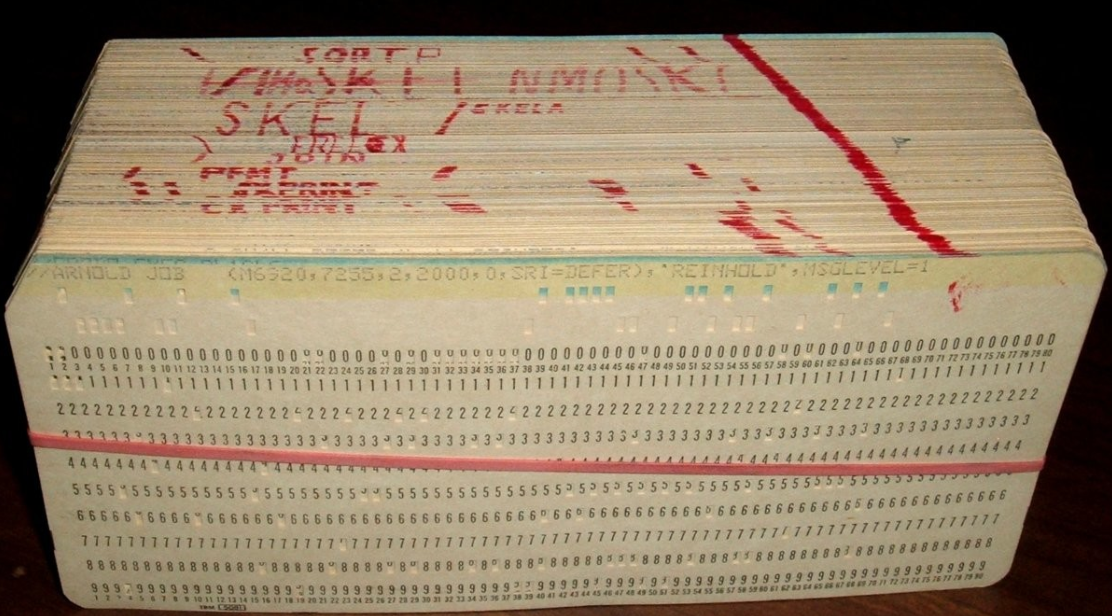
\includegraphics[width=0.6\linewidth]{Imagenes/tarjetas.png}
	\caption{Una pila de tarjetas perforadas, que podían contener un conjunto de instrucciones.}
	\label{fig:enter-label}
\end{figure}

\subsection{La segunda generación (1955 a 1965): los transistores}

La llegada de los transistores a mediados de la década de los 50 lo cambió todo. Este evento permitió la construcción de computadoras más pequeñas, además de ser mucho más eficientes, los transistores consumían mucho menos energía. Los transistores aumentaron la velocidad de procesamiento, permitiendo realizar operaciones mucho más rápidas, finalmente los transistores popularizaron los equipos de cómputo al reducir el costo de fabricación.

\begin{figure}[H]
	\centering
	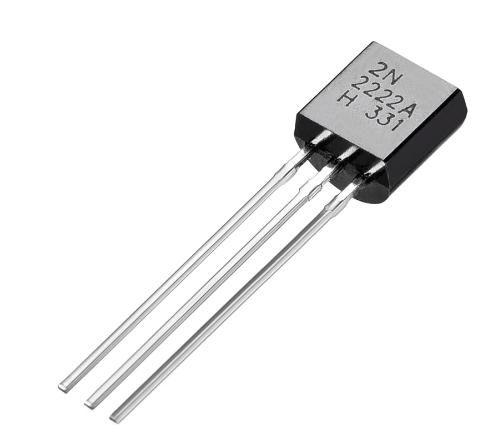
\includegraphics[width=0.4\linewidth]{Imagenes/transistor.png}
	\caption{Los transistores permitieron la fabricación de computadoras más compactas y portátiles.}
	\label{fig:enter-label}
\end{figure}

En 1957 surge FORTRAN (FORmula TRANslation), uno de los primeros lenguajes de programación de alto nivel desarrollado por IBM.

FORTRAN revolucionó la programación, haciendo más accesible el uso de computadoras para científicos e ingenieros y estableciendo estándares que influenciarían futuros lenguajes de programación.

\begin{figure}[H]
	\centering
	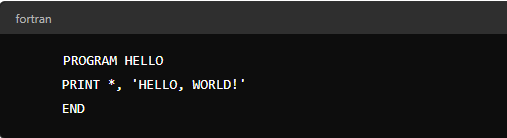
\includegraphics[width=0.8\linewidth]{Imagenes/fortran.png}
	\caption{Ejemplo de programa escrito con FORTRAN.}
	\label{fig:enter-label}
\end{figure}
Durante esta época, surgen  los primeros sistemas operativos, para  gestionar mejor los recursos de la computadora y ejecutar programas como los escritos en FORTRAN.





\subsection{La tercera generación (1965 a 1980): los circuitos integrados}

La introducción de los circuitos integrados (IC) en la década de 1960 revolucionó la industria de la computación. Estos componentes permitieron construir computadoras aún más pequeñas, rápidas y eficientes al integrar múltiples transistores en un solo chip. La reducción del tamaño y costo, junto con el aumento en la capacidad de procesamiento, hizo que las computadoras fueran más accesibles para empresas y universidades.

\begin{figure}[H]
	\centering
	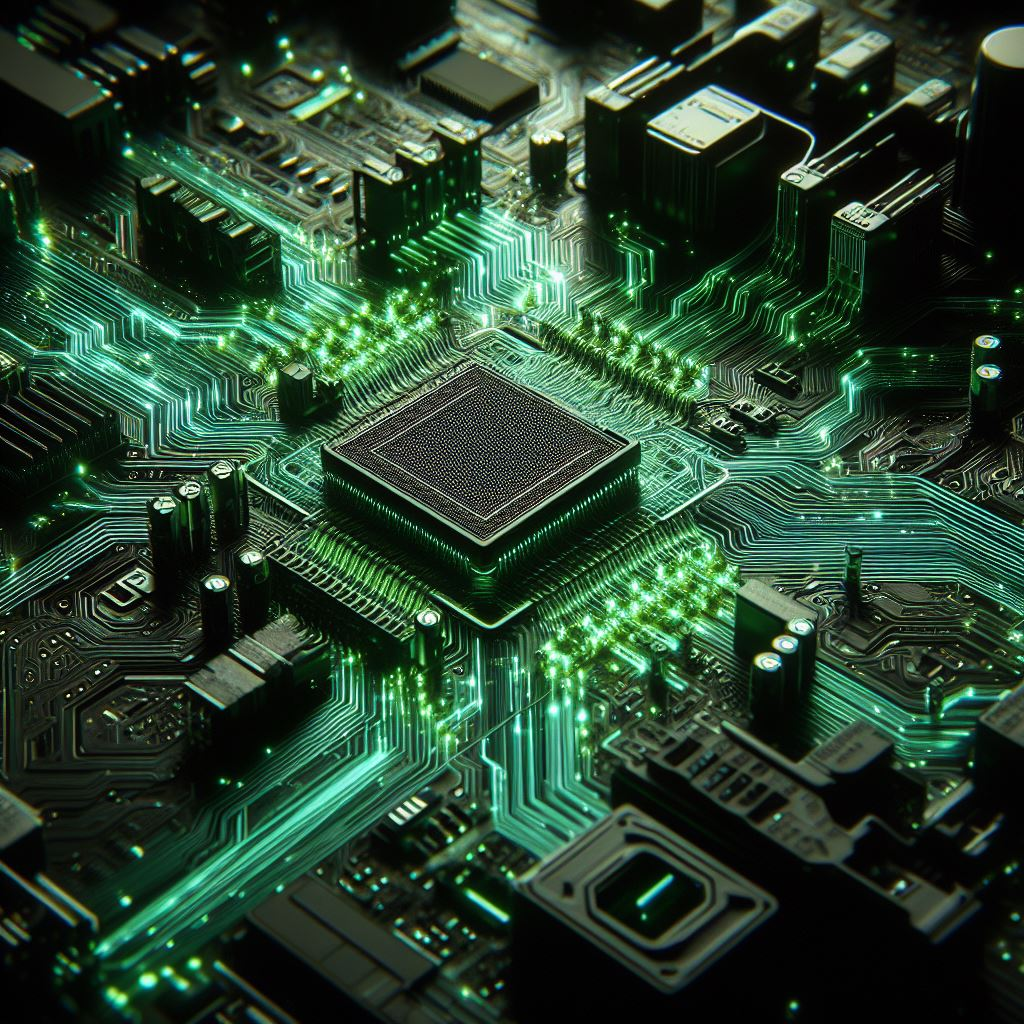
\includegraphics[width=0.4\linewidth]{Imagenes/buses.jpeg}
	\caption{Los circuitos integrados dar un salto en potencia y complejidad a los computadores.}
	\label{fig:enter-label}
\end{figure}

Durante esta generación, los sistemas operativos evolucionaron significativamente. Surgieron conceptos como la multiprogramación, que permitía que múltiples programas se ejecutaran al mismo tiempo, mejorando la utilización de la CPU. También se desarrollaron los sistemas de tiempo compartido, que permitían a múltiples usuarios interactuar con la computadora simultáneamente, lo que optimizó el uso de los recursos y facilitó el acceso a la computación.

Los lenguajes de programación de alto nivel continuaron evolucionando, y COBOL (Common Business-Oriented Language) se popularizó en el ámbito empresarial. Este lenguaje facilitó la programación de aplicaciones de gestión y negocios, ampliando el alcance de las computadoras en el sector comercial.

\subsection{La cuarta generación (1980 a la fecha): las computadoras personales}


La cuarta generación de computadoras comenzó en la década de 1980 con la aparición de los microprocesadores, que integraron la CPU completa en un solo chip. Esto permitió la creación de computadoras personales (PC) asequibles y potentes, accesibles para el uso doméstico y empresarial.
\begin{figure}[H]
	\centering
	
\includegraphics[width=0.4\linewidth]{Imagenes/computer.png}
	\caption{Desde los 80 en adelante, se popularizan las computadoras personales.}
	\label{fig:enter-label}
\end{figure}

Durante esta generación, los sistemas operativos avanzaron enormemente. Surgieron sistemas operativos gráficos como Windows y macOS, que hicieron que las computadoras fueran más fáciles de usar y accesibles para el público en general. La multitarea se convirtió en una característica estándar, permitiendo a los usuarios ejecutar múltiples aplicaciones simultáneamente.

La conectividad a internet se volvió omnipresente, transformando la forma en que las computadoras se utilizan para la comunicación, el comercio y el entretenimiento. Surgieron nuevas tecnologías como la computación en la nube, que permitieron el acceso remoto a recursos y servicios, y la inteligencia artificial, que comenzó a integrarse en diversas aplicaciones.

La popularización de los dispositivos móviles, como los smartphones y las tabletas, también marcó esta era, extendiendo las capacidades de las computadoras personales a dispositivos más portátiles y versátiles.




\section{Técnicas de mejora de rendimiento utilizadas en los sistemas operativos}
A medida que los sistemas operativos evolucionaban, se desarrollaron técnicas avanzadas para optimizar el uso de los recursos de hardware. Estas técnicas permitieron un mejor rendimiento y eficiencia en la gestión de tareas y recursos. Entre ellas se encuentran:

\subsection{Offline Processing}

\textbf{Descripción:} Permite procesar trabajos en lotes sin intervención del usuario. Los trabajos se preparan y almacenan para ser ejecutados posteriormente, optimizando el uso del tiempo de la CPU y otros recursos del sistema.

\textbf{Ejemplo:} Actualizaciones de Windows programadas para ejecutarse durante la noche.

\subsection{Buffering}
\textbf{Descripción:} Utiliza una memoria intermedia (buffer) para almacenar temporalmente datos durante las operaciones de entrada/salida (E/S). Esto permite que la CPU y los dispositivos de E/S trabajen de manera más eficiente y simultánea.

\textbf{Funcionamiento:} Mientras el dispositivo de E/S procesa un bloque de datos, la CPU puede seguir trabajando con otros datos almacenados en el buffer.

\textbf{Ejemplo: }Al ver un video en streaming, los datos se almacenan en un buffer antes de ser reproducidos, asegurando una reproducción continua sin interrupciones.

\subsection{Spooling (Simultaneous Peripheral Operations On-Line)}

\textbf{Descripción:} Almacena trabajos de E/S en una cola en el disco para ser procesados secuencialmente. Es especialmente útil para dispositivos que no pueden manejar múltiples tareas simultáneamente, como las impresoras.

\textbf{Funcionamiento:} Los documentos enviados a imprimir se almacenan en una cola en el disco (spool) y la impresora los procesa uno a uno en el orden en que llegaron.

\textbf{Ventajas:} Mejora la utilización de dispositivos periféricos, reduce el tiempo de espera y permite una gestión ordenada de los trabajos.

\textbf{Ejemplo:} En una oficina, varios usuarios envían trabajos de impresión simultáneamente. La técnica de spooling permite que estos trabajos se gestionen de manera eficiente y sin conflicto.

\section{Multiprogramación}
La multiprogramación es una técnica en la cual un sistema operativo permite que múltiples programas se ejecuten simultáneamente en una computadora. Esto se logra compartiendo el tiempo de la CPU entre varios programas, de modo que mientras un programa está esperando una operación de entrada/salida (como leer datos del disco), otro programa puede usar la CPU.

\subsection{Características de la Multiprogramación:}
\subsubsection{Maximización del Uso de la CPU}La CPU nunca está inactiva, siempre tiene trabajo que hacer.
\subsubsection{Gestión de Recursos:} La memoria, el almacenamiento y los dispositivos de E/S se gestionan de manera eficiente para que varios programas puedan ejecutarse sin interferencias.
\subsubsection{Context Switching:} El sistema operativo cambia rápidamente entre programas, lo que permite que varios programas parezcan ejecutarse al mismo tiempo.

\textbf{Ejemplos}

\textbf{Sistema Bancario:} Un banco puede procesar múltiples transacciones simultáneamente. Mientras una transacción espera la confirmación de una operación, otra transacción puede ser procesada.

\textbf{Uso Personal:} En una computadora personal, puedes escuchar música, descargar un archivo y escribir un documento al mismo tiempo gracias a la multiprogramación.

La multiprogramación es una base fundamental de los sistemas operativos modernos, permitiendo una utilización más eficiente y efectiva de los recursos de la computadora.

\section{Tiempo compartido (Time sharing)}
El tiempo compartido es una técnica de gestión de recursos en sistemas operativos que permite que múltiples usuarios utilicen una computadora simultáneamente. Esto se logra dividiendo el tiempo de la CPU en pequeños segmentos y asignando cada segmento a diferentes tareas o usuarios. Aquí están los puntos clave:
\begin{itemize}
	\item \textbf{Multiplicidad de usuarios:}  Varios usuarios pueden interactuar con el sistema al mismo tiempo.
	\item \textbf{Interactividad:}  Proporciona respuestas rápidas a cada usuario, creando la ilusión de acceso exclusivo.
	\item  \textbf{Gestión de recursos:} El sistema operativo gestiona la asignación de CPU, memoria y dispositivos de E/S entre las tareas.
\end{itemize}
\subsection{Funcionamiento}
\begin{itemize}
	\item \textbf{Slices de Tiempo}: La CPU se divide en pequeños intervalos de tiempo llamados "slices" o "quantums".
	\item \textbf{Asignación}: Cada usuario o tarea recibe un slice de tiempo, y la CPU alterna rápidamente entre ellos.
	\item \textbf{Interrupciones}: Al finalizar el slice de tiempo, una interrupción cambia el control de la CPU al siguiente usuario o tarea en cola.
\end{itemize}

\section{Tiempo real (Real time)}
El tiempo real en sistemas operativos se refiere a la capacidad de procesar datos y eventos de forma inmediata o dentro de un plazo específico y predecible. Los sistemas de tiempo real están diseñados para aplicaciones donde es crucial que las respuestas se entreguen sin demoras significativas. Aquí están los puntos clave:

\begin{itemize}
	\item \textbf{Determinismo}: Garantiza que las tareas se completen dentro de un tiempo específico.
	\item \textbf{Prioridades}: Asigna prioridades a las tareas, asegurando que las de mayor importancia se procesen primero.
	\item \textbf{Ejemplos}: Control de sistemas industriales, aviación, telecomunicaciones, y dispositivos médicos.
\end{itemize}
\section{Proceso distribuido}
Un proceso distribuido se refiere a un sistema en el que múltiples computadoras trabajan juntas para completar tareas o resolver problemas. Este enfoque distribuye la carga de trabajo entre varias máquinas, mejorando la eficiencia y la capacidad de procesamiento.

\subsection{Características}
\begin{itemize}
	\item \textbf{Descentralización}: No hay un único punto de control, lo que aumenta la robustez y la fiabilidad del sistema.
	\item \textbf{Concurrencia}: Múltiples procesos pueden ejecutarse simultáneamente en diferentes máquinas.
	\item \textbf{Escalabilidad}: Es fácil agregar más computadoras para aumentar la capacidad de procesamiento.
	\item \textbf{Fallo Tolerante}: Si una máquina falla, las otras pueden continuar con el trabajo, mejorando la resiliencia.
\end{itemize}

\subsection{Ejemplos}
\begin{itemize}
	\item \textbf{Sistemas de Archivos Distribuidos}: Almacenan datos en varias computadoras, permitiendo acceso rápido y redundante.
	\item \textbf{Computación en la Nube}: Proveedores como AWS, Google Cloud y Azure utilizan procesos distribuidos para ofrecer servicios de alta disponibilidad y escalabilidad.
	\item \textbf{Aplicaciones Web}: Sitios web de alto tráfico utilizan múltiples servidores para manejar solicitudes simultáneas y mejorar el rendimiento.
\end{itemize}

\section{Multiproceso}
El multiproceso es una técnica utilizada en sistemas operativos que permite ejecutar múltiples procesos simultáneamente utilizando más de una unidad central de procesamiento (CPU) o núcleo de CPU. Esto mejora significativamente el rendimiento y la eficiencia del sistema.

\subsection{Características}
\begin{itemize}
	\item \textbf{Paralelismo}: Los procesos se ejecutan en paralelo, utilizando múltiples CPUs o núcleos.
	\item \textbf{Independencia}: Cada proceso puede ejecutarse de manera independiente, sin afectar a los demás.
	\item \textbf{Escalabilidad}: Añadir más CPUs o núcleos mejora el rendimiento del sistema.
\end{itemize}

\subsection{Ventajas}
\begin{itemize}
	\item \textbf{Mejora del Rendimiento}: Permite realizar múltiples tareas al mismo tiempo, aumentando la velocidad de procesamiento.
	\item \textbf{Mayor Eficiencia}: Utiliza mejor los recursos del sistema, distribuyendo la carga de trabajo entre varias CPUs.
\end{itemize}

\subsection{Ejemplos}
\begin{itemize}
	\item \textbf{Servidores Web}: Manejan múltiples solicitudes de usuarios simultáneamente.
	\item \textbf{Aplicaciones Científicas}: Realizan cálculos complejos en paralelo, acelerando el tiempo de procesamiento.
	\item \textbf{Juegos y Software de Diseño}: Utilizan múltiples núcleos para gráficos y cálculos intensivos.
\end{itemize}

\subsection*{Comparación con la Multiprogramación}
\begin{itemize}
	\item \textbf{Multiprogramación}: Utiliza una sola CPU para ejecutar múltiples tareas, alternando rápidamente entre ellas.
	\item \textbf{Multiproceso}: Utiliza múltiples CPUs o núcleos para ejecutar tareas en paralelo, lo que permite un verdadero procesamiento simultáneo.
\end{itemize}

